% -*- TeX:de -*-
\NeedsTeXFormat{LaTeX2e}
\documentclass[12pt,a4paper]{article}
\usepackage[german]{babel} % german text
\usepackage[DIV12]{typearea} % size of printable area
\usepackage[T1]{fontenc} % font encoding
%\usepackage[latin1]{inputenc} % most likely on Windows
\usepackage[utf8]{inputenc} % probably on Linux
\usepackage{multicol}

% PLOTTING
\usepackage{pgfplots} 
\usepackage{pgfplotstable}
\usepackage{url}
\usepackage{graphicx} % to include images
\usepackage{tikz}
\usepackage{subfigure} % for creating subfigures
\usepackage{amsmath} % a bunch of symbols
\usepackage{amssymb} % even more symbols
\usepackage{booktabs} % pretty tables
\usepackage{makecell} % multi row table heading

% a floating environment for circuits
\usepackage{float}
\usepackage{caption}

%\newfloat{circuit}{tbph}{circuits}
%\floatname{circuit}{Schaltplan}

% a floating environment for diagrams
%\newfloat{diagram}{tbph}{diagrams}
%\floatname{diagram}{Diagramm}

\selectlanguage{german} % use german

\begin{document}








%%%% TO DO
%
% - - Shorty:
%
% - - Tabelle "Messwerte Linsenbrennweite"
%		bitte bei jedem neuen e eine trennlinie... bin zu deppert ^^

% - - Patrick
%




%%%%%%% DECKBLATT %%%%%%%
\thispagestyle{empty}
			\begin{center}
			\Large{Fakultät für Physik}\\
			\end{center}
\begin{verbatim}


\end{verbatim}
							%Eintrag des Wintersemesters
			\begin{center}
			\textbf{\LARGE WS 2013/14}
			\end{center}
\begin{verbatim}


\end{verbatim}
			\begin{center}
			\textbf{\LARGE{Physikalisches Praktikum\\ für das Bachelorstudium}}
			\end{center}
\begin{verbatim}




\end{verbatim}

			\begin{center}
			\textbf{\LARGE{PROTOKOLL}}
			\end{center}
			
\begin{verbatim}





\end{verbatim}

			\begin{flushleft}
			\textbf{\Large{Experiment (Nr., Titel):}}\\
							%Experiment Nr. und Titel statt den Punkten eintragen
			\LARGE{PW9 Gleichstrom}	
			\end{flushleft}

\begin{verbatim}

\end{verbatim}	
							%Eintragen des Abgabedatums, oder des Erstelldatums des Protokolls
			\begin{flushleft}
			\textbf{\Large{Datum:}} \Large{21.11.2013}
			\end{flushleft}
			
\begin{verbatim}
\end{verbatim}
							%Namen der Protokollschreiber
		\begin{flushleft}
			\textbf{\Large{Namen:}} \Large{Patrick Braun, Johannes Kurz}
			\end{flushleft}

\begin{verbatim}


\end{verbatim}
							%Kurstag und Gruppennummer, zb. Fr/5
			\begin{flushleft}
			\textbf{\Large{Kurstag/Gruppe:}} \Large{DO/2}
			\end{flushleft}

\begin{verbatim}



\end{verbatim}
							%Name des Betreuers, das Praktikum betreute.
			\begin{flushleft}
			\LARGE{\textbf{Betreuer:}}	\Large{ Clemens Nagel }	
			\end{flushleft}

%%%%%%% DECKBLATT ENDE %%%%%%%
\pagebreak
\setlength{\columnsep}{20pt}
\begin{multicols}{2}

%%%%%%%%%%%%%%%%%%%%%%%%%%%%%%%%%%%%%%%%%%%%%%%%
%\end{multicols}
%\begin{figure}[H]
%	\centering
%	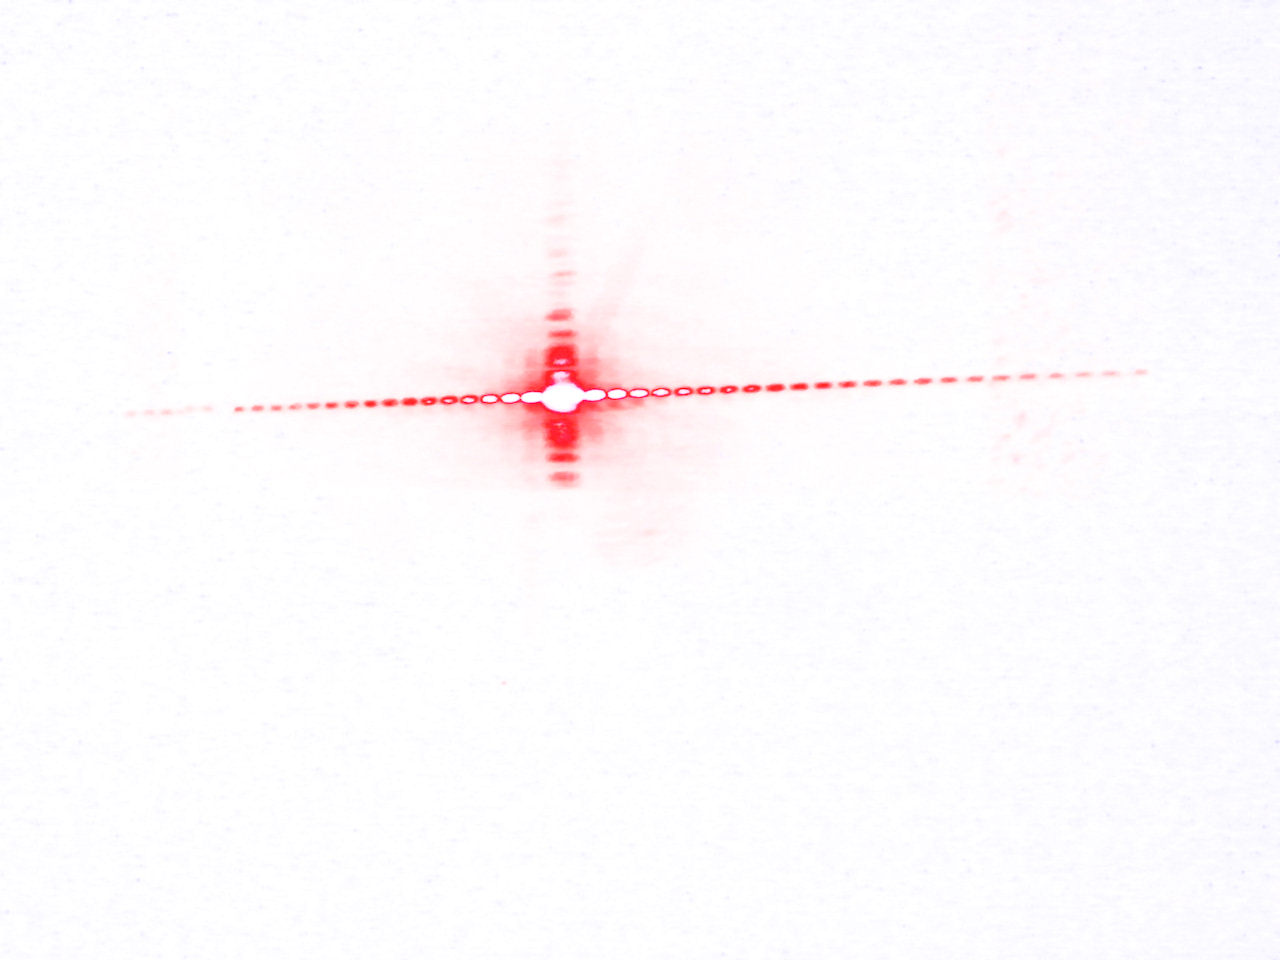
\includegraphics[scale=0.35]{./figure/beugung.png}
%	\caption{Beugungsmuster Einzelspalt (echtes Foto; schwarz durch weiß ersetzt)}
%	\label{fig:beugungsmuster}
%\end{figure}

\begin{multicols}{2}

\section{Beugung am Spalt und Doppelspalt}
\subsection{Messwerte und Ergebnisse}

%\begin{figure}[H]
%	\centering
%	\pgfplotstabletypeset[
%			columns={abstand, n},
%			col sep=&,
%			columns/abstand/.style={precision=2, zerofill, column name=\makecell{$Abstand$\\$(\pm 0.05)[mm]$} }, 
%			columns/n/.style={column name=\makecell{$n$\\$(Ordnung)$}, precision=0},
%			every head row/.style={before row=\hline,after row=\hline\hline},
%			every last row/.style={after row=\hline},
%			every first column/.style={column type/.add={|}{} },
%			every last column/.style={column type/.add={}{|} }
%			]{
%			abstand & n
%			12.9 & 1
%			24.45 & 2
%			37.40 & 3
%			49.35& 4
%			62.45 & 5
%			74.45 & 6
%			87.45 & 7
%			100.25 & 8
%			
%			}
%	\caption{Messwerte Einzelspalt}
%	\label{tab:werte_einzelspalt}
%\end{figure}
%
\subsection{Diskussion}
%%%%%%%%%%%%%%%%%%%%%%%%%%%%%%%%%%%%%%%%%%%%%%%%
\section{Wellenlängenmessung am Gitter}

\subsection{Messwerte und Ergebnisse}

\subsection{Diskussion}
%%%%%%%%%%%%%%%%%%%%%%%%%%%%%%%%%%%%%%%%%%%%%%%%
\section{Newtonsche Ringe}

Die Newtonringe sind ein Inteferenzbild von Licht, dass durch eine sehr schwach gekrümmte plan-konvexe Linse fällt, an die direkt eine Glasplatte anschließt. Zwischen Platte und Linse ist also, abgesehen vom Berührungspunkt, ein kurzer Abschnitt Luft, der, dank der schwachen Krümmung der Linse, nahezu ein rechtwinkeliges Dreieck bildet (siehe Abb. \ref{fig:newtonringe_reflexion}).\\


\begin{figure}[H]
	\centering
	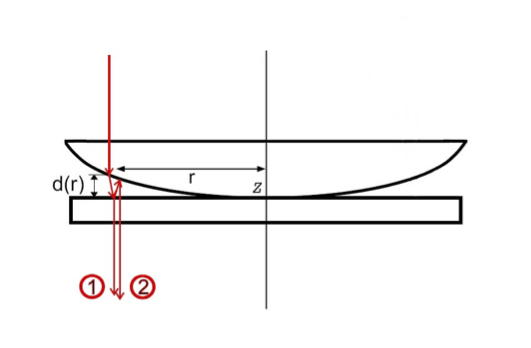
\includegraphics[scale=0.80]{./figure/newtonringe_strahlengang.png}
	\caption{Strahlengang in Transmission}
	\label{fig:newtonringe_transmission}
\end{figure}


Durch den Unterschied im Brechungsindex, zwischen Glas und Luft und durch teilweise Reflexion, werden aus jedem einfallenden Strahl eine Vielzahl (nahezu) paralleler Strahlen mit leicht unterschiedlichen Phasen. Aus der Überlagerung der Erzeugnisse aller einfallender Strahlen ergeben sich schließlich die beobachtbaren Newtonringe, ein Inteferenzmuster.\\
Das gleiche Prinzip gilt auch für die Strahlen, die reflektiert werden und durch die Linse wieder austreten. Auch hier entstehen fast-parallele Strahlen mit Phasenunterschieden.\\
Um den Effekt schön zu erzielen, ist Licht mit ausreichend großer Kohärenzlänge nötig. In diesem Versuch wird eine Halogenlampe verwendet.
\\
Das Licht aus der Lampe fällt auf das System aus Linse und Glasplatte. Unter Verwendung 2er Strahlteiler und Sammellinsen werden sowohl die Newtonringe in Reflexion, als auch die in Transmission, direkt nebeneinander auf einen Schirm projiziert (Abb. \ref{fig:newtonringe_aufbau}).

\begin{figure}[H]
	\centering
	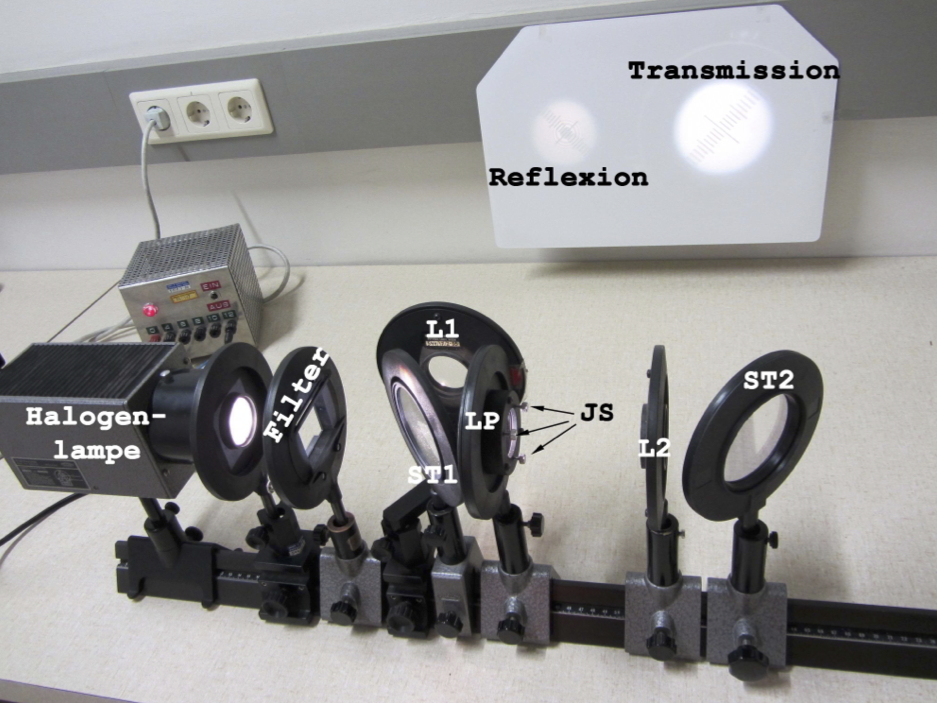
\includegraphics[scale=0.45]{./figure/newtonringe_aufbau.png}
	\caption{Versuchsaufbau - Newtonringe}
	\label{fig:newtonringe_aufbau}
\end{figure}

\noindent $Strahlteiler: ST1, ST2$\\
$Sammellinsen: L1, L2$\\
$Linse-Glasplatte: LP$\\
\\
Wird der Versuchsaufbau ohne Farbfilter eingeschaltet, lassen sich die Newtonringe zwar gut als solche erkennen, jedoch nicht eindeutig begrenzen. Die verschiedenen Spektralfarben werden unterschiedlich stark "abgelenkt": Die unterschiedlichen Wellenlängen bewirken, dass die Phasenverschiebungen verschiedene Minima und Maxima für verschiedene Spektralfarben erzeugen. Dadurch verschmieren die Ringe.\\
Je weiter außen sie betrachtet werden, desto unschärfer wird das Bild.\\
Durch den Farbfilter wird eine Wellenlänge herausgegriffen. Das verringert die Intensität deutlich, führt jedoch zu einer sehr viel klareren Abgrenzung der einzelnen Ringe voneinander.\\
der hier verwendete Farbfilter:\\
grün: $\lambda = (518 \pm 3) nm$\\
\\
Aus geometrischen Betrachtungen ergibt sich für den Zusammenhang zwischen dem Radius $r$ der Newtonringe und dem Krümmungsradius $R$ der Linse:
$$r^2 = (2R-d)d$$
$d$... Abstand zwischen Linse und Platte\\
Auslöschung liegt im reflektierten Fall vor, wenn:
$$2d_k + \frac{\lambda}{2}=(2k+1)(\frac{\lambda}{2})$$
Da $R$ sehr viel größer ist als $d$ gilt also für Auslöschungen im Reflexionsfall:
$$r_k^2 =kR\lambda$$
konstruktive Interferenz:
$$r_k^2=(2k+1R \frac{\lambda}{2})$$
Im Fall der Ringe in Transmission gelten beide Gleichungen für die jeweils andere Art von Interferenz.\\
\\
Der Krümmungsradius $R$ soll bestimmt werden, indem die Radien $r_k$ verschiedener Maxima bzw. Minima in beiden Interferenzbildern gemessen werden um so R in linearer Regression zu ermitteln:
$$R=\frac{r_k^2}{k \lambda}$$

\noindent Die Inteferenzringe werden auf ein Blatt Papier projiziert, markiert und anschließend mit einer Schublehre vermessen.
Dazu ist außerdem auf der Glasplatte des Systems ein mm-Maßstab angebracht, der es erlaubt, die Größenverhältnisse der Abbildung zu bestimmen.

\subsection{Messwerte und Ergebnisse}

Umrechnungsfaktor Reflexion: $\frac{5}{18}$\\
\indent $18mm_{Messung} = 5mm_{wirklich}$\\
Transmission: $\frac{1}{5}$\\
\indent $25mm_{Messung} = 5mm_{wirklich}$\\
\\
Wellenlänge: $\lambda = (518\pm 3)nm$

\begin{figure}[H]
	\centering
	\pgfplotstabletypeset[
			columns={reflex, transmiss},
			col sep=&,
			columns/reflex/.style={column name=\makecell{Radius $r_k$\\Reflexion\\$[mm]$\\ $\pm 0.1mm$} }, 
			columns/transmiss/.style={column name=\makecell{Radius $r_k$\\Transmission\\ $[mm]$\\ $\pm 0.1mm$}}, 
			every head row/.style={before row=\hline,after row=\hline\hline},
			every last row/.style={after row=\hline},
			every first column/.style={column type/.add={|}{} },
			every last column/.style={column type/.add={}{|} }
			]{
			reflex & transmiss
			%6.2 & 
%			10.5 & 13.6
%			14.3 & 19.4
%			17.0 & 23.1
%			19.8 & 26.1
%			22.2 & 29.4
%			24.1 & 32.0
			
			1.7 & 2.7
			2.9 & 3.9
			4.0 & 4.6
			4.7 & 5.2
			5.6 & 5.9
			6.2& 6.4
			6.7 & 			
			
			
			}
	\caption{gemessene Radien der Newtonringe}
	\label{fig:radien_newtonringe}
\end{figure}



\end{multicols}
\begin{figure}[H]
	\centering
	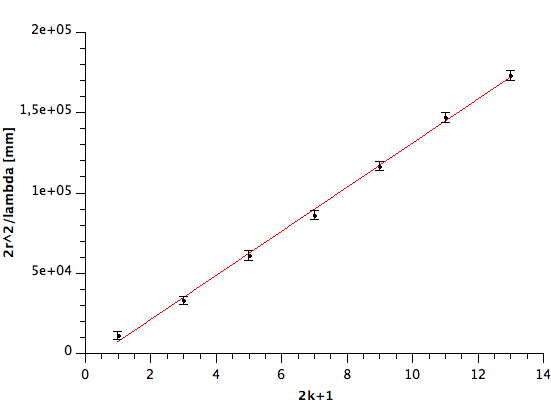
\includegraphics[scale=0.60]{./figure/newtonringe_reflex_regress.png}
	\caption{Newtonringe - Reflexion: $R=2r_k^2*\frac{1}{\lambda (2k+1)}$}
	\label{fig:newtonringe_reflex_regress}
\end{figure}

%Aus der Steigung: R der Linse
$$R_{Reflexion} = 13.73 \pm 0.27)m$$



\begin{figure}[H]
	\centering
	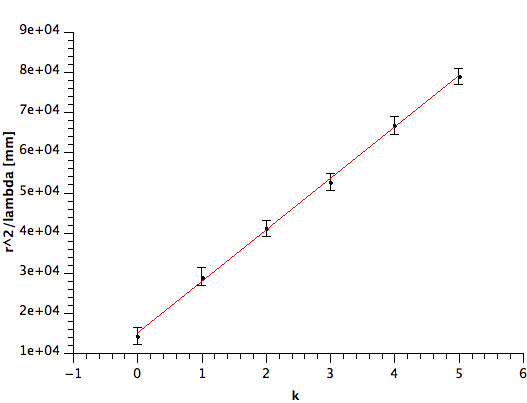
\includegraphics[scale=0.60]{./figure/newtonringe_transmiss_regress.png}
	\caption{Newtonringe - Transmission: $R=r_k^2\frac{1}{\lambda *k}$}
	\label{fig:newtonringe_transmiss_regress}
\end{figure}

$$R_{Transmission}=(12.82 \pm 0.87)m$$

%B (y-intercept) = 1,509918148328588e+04 +/- 2,520381237651498e+03
%A (slope) = 1,281922284232692e+04 +/- 8,668173766933726e+02
\begin{multicols}{2}

\subsection{Diskussion}

Der Krümmungsradius $R$ aus den Messungen der Reflexions-Newtonringe stimmt sehr genau mit den Angaben der Betreuerin überein (etwa 13.7 m). Die Abweichung der einzelnen Messpunkte von der Regressionsgerade ist klein und auch die einzelnen Unsicherheiten auf der y-Achse konnten klein abgeschätzt werden (Abb. \ref{fig:newtonringe_reflex_regress}).
\\
(Die Unsicherheit von $\lambda$ ist vorgegeben, die der gemessenen Radien mit dem doppelten der Auflösung der Schublehre -$\pm 0.1 mm$ -  vorsichtig gewählt)
\\
\\
Die Messung der aus den Transmissions-Ringen ist etwas problematischer:\\
Zwar liegt das Ergebnis durchaus in der Nähe des erwarteten Wertes, die einzelnen Messwerte schwanken jedoch deutlich, im Vergleich zur anderen Messung. Das führt zu einer fast 4mal größeren Unsicherheit (Abb. \ref{fig:newtonringe_transmiss_regress}).\\
Schon das Markieren der Ringe am Papier hat erwarten lassen, dass diese Messung ungenauer ist. Die hellen Ringe aus der Transmission waren deutlich schwieriger zu erkennen und weniger eindeutig.\\
Teil der Aufgabenstellung ist die Frage nach dem Kontrast zwischen hellen und dunklen Ringen, der im transmittierten Inteferenzbild schwächer sein soll, als im reflektierten:\\
Da weniger Licht an einer Grenzfläche reflektiert wird, als durchgeht, ist der Kontrast im Transmissionsfall (2 Reflexionen, siehe Abb. \ref{fig:newtonringe_transmission}) viele geringer, als im Reflexionsfall (nur 1 Reflexion).\\
Dieser Effekt hat zur Schwierigkeit der Messung wesentlich beigetragen, und erklärt, zumindest teilweise, das ungenauere Ergebnis im Transmissionsfall.\\
\\
Die Vergrößerung der transmittierten Abbildung ist leicht größer, was zu einer Verkleinerung der Messunsicherheit führt. Die ist jedoch klein gegen die Ungenauigkeiten durch weniger Intensität und unklare Ringgrenzen.\\
\\
Der Versuch ließe sich vielleicht durch eine stärkere Lampe noch genauer durchführen. Umständlicher aber auch effektiv wäre womöglich ein vertikaler Aufbau, um die Markierung flach auf dem Tisch durchführen zu können oder zumindest eine stabile Wand als Schirm zu verwenden.\\
Die erzielten Ergebnisse sind jedoch gut am erwarteten Wert.

\section{Quellen}
$[1]$ Leitfaden, \url{http://www.univie.ac.at/anfpra/neu1/pw/pw8/PW8.pdf}\\
$[2]$ Quecksilberdampflampe, \url{http://de.wikipedia.org/wiki/Quecksilberdampflampe}\\
%$[2]$

\end{multicols}

\begin{figure}[H]
	\centering
	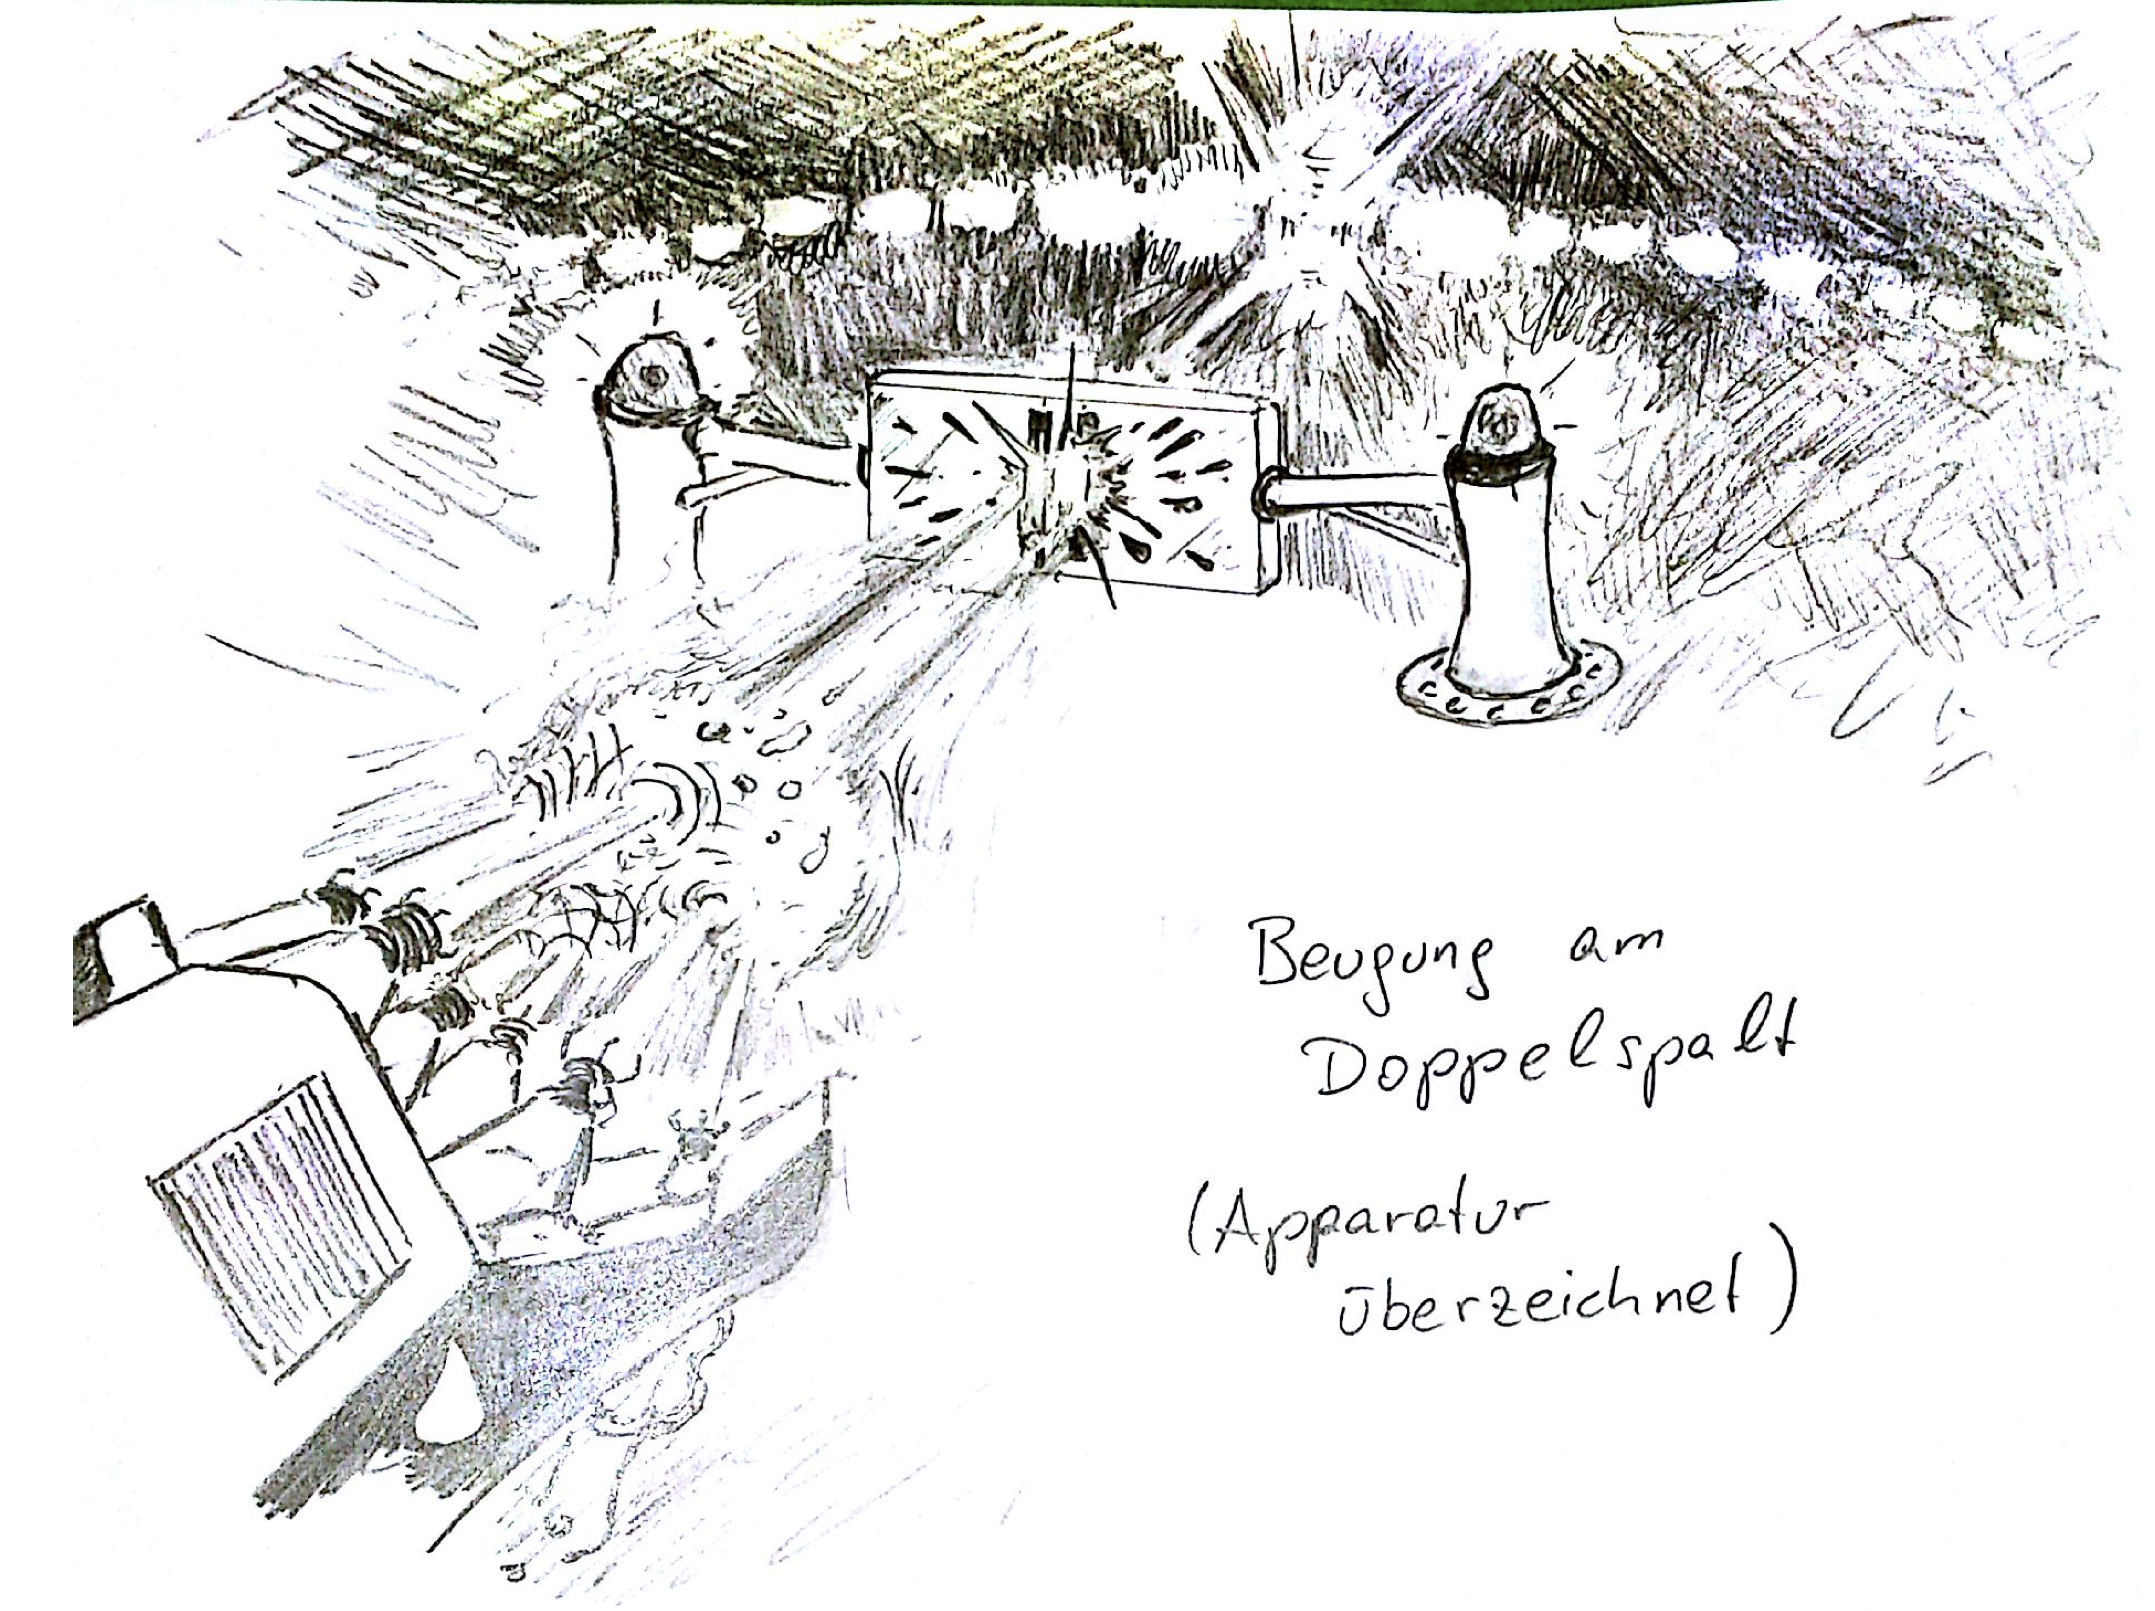
\includegraphics[scale=0.65]{./figure/laser_kanone.png}
	\caption{Beugung am Doppelspalt}
	\label{fig:laser_kanone}
\end{figure}

\end{document}